Jets are used to monitor both the EM and hadronic calorimeter.
These jets consist of grouping of EM and hadronic clusters.
The \antikt{} jet-finding algorithm, which is described in Section \ref{sec:Theory:Jets}, is used with an $R=0.4$ for the offline jets.
Only offline jets with a $\pt{}>20$ GeV are considered, which is the same as the analysis selection.
The L2 jet-finding is done using a cone algorithm.
The cone algorithm is seeded using a L1 RoI, and all deposits within the radius of the cone are combined, and a new cone centre is defined using the energy weighted position of the constituents.
With the new cone defined, any new deposits within the radius are again combined, and a new cone centre is defined.
This continues until the cone centre does not change.

The \antikt{} jet-finding algorithm is used for the EF jets. 
While it is the same jet-finding algorithm, the EF jets run over clusters that are close to the RoI.
In the 2012 data taking, calibration is applied to the EF jets to account for the non-compensating calorimeters. 

\subsubsection{Jet matching}

The trigger jets are matched to offline jets using \dr{} to allow them to be compared.
Figure \ref{SW_jet_L2_dR} shows the \dr{} between the offline jets and all L2 jets in the event.
As observed in the EM clusters, in (a) there are two peaks; one at $\dr{}\approx0$ and one at $\dr{}\approx\pi$.
The differences from the EM clusters are best seen in (b), the first peak is not quite at zero.
This is due to the $\phi$ resolution of the jets shifting the \dphi{} away from zero. 
Figure \ref{SW_jet_EF_dR} shows the \dr{} between the offline jets and all EF jets in the event.
The distributions are similar to the L2 jet \dr{} distributions, with a peak just above zero, and one at $\dr{}\approx\pi$. 

A matching selection of $\dr{}<0.4$ is used for both the L2 and EF jets.
This corresponds to the R value used in the jet-finding for both the trigger and offline jets.

\begin{figure}
\centering
        \begin{subfigure}[b]{0.5\textwidth}
                \centering
                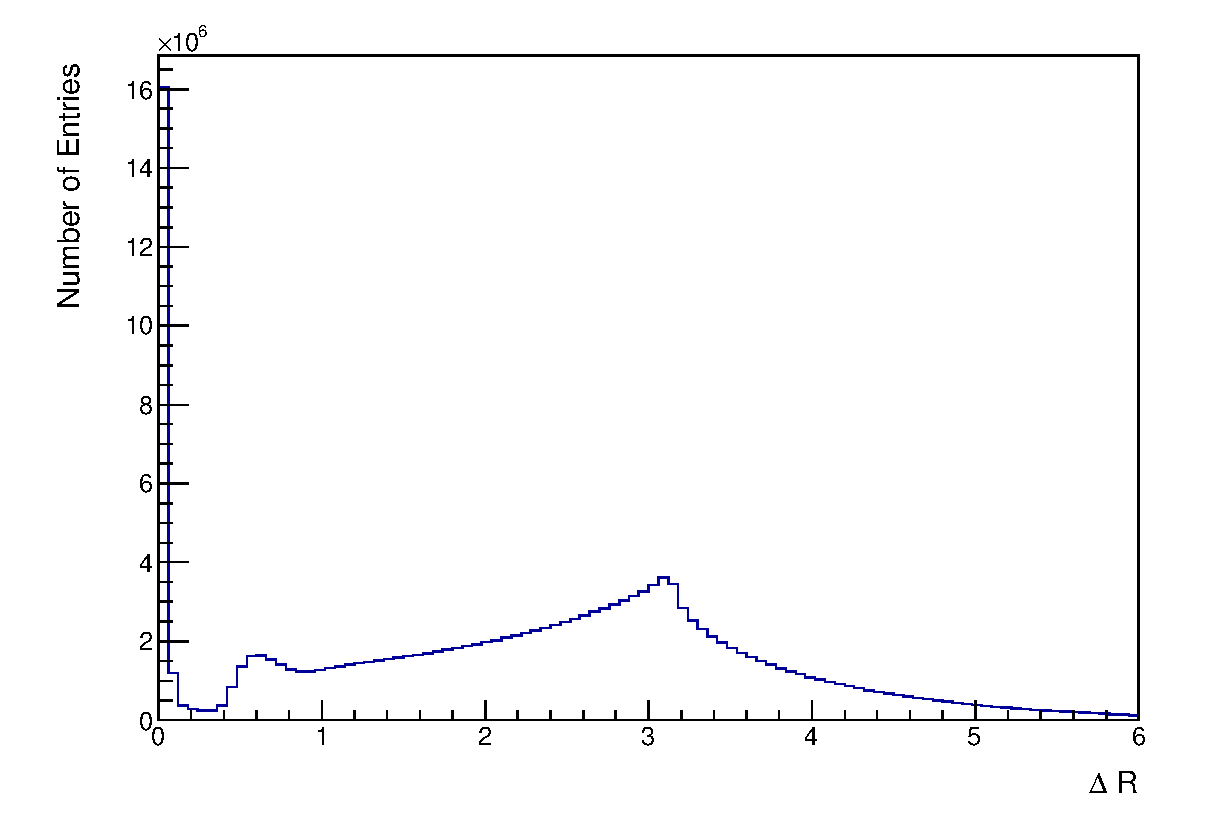
\includegraphics[width=\textwidth]{figures/ServiceWork/Jets/L2_DRUnmatchedJetsJet.eps}
        \end{subfigure}%
        \begin{subfigure}[b]{0.5\textwidth}
                \centering
                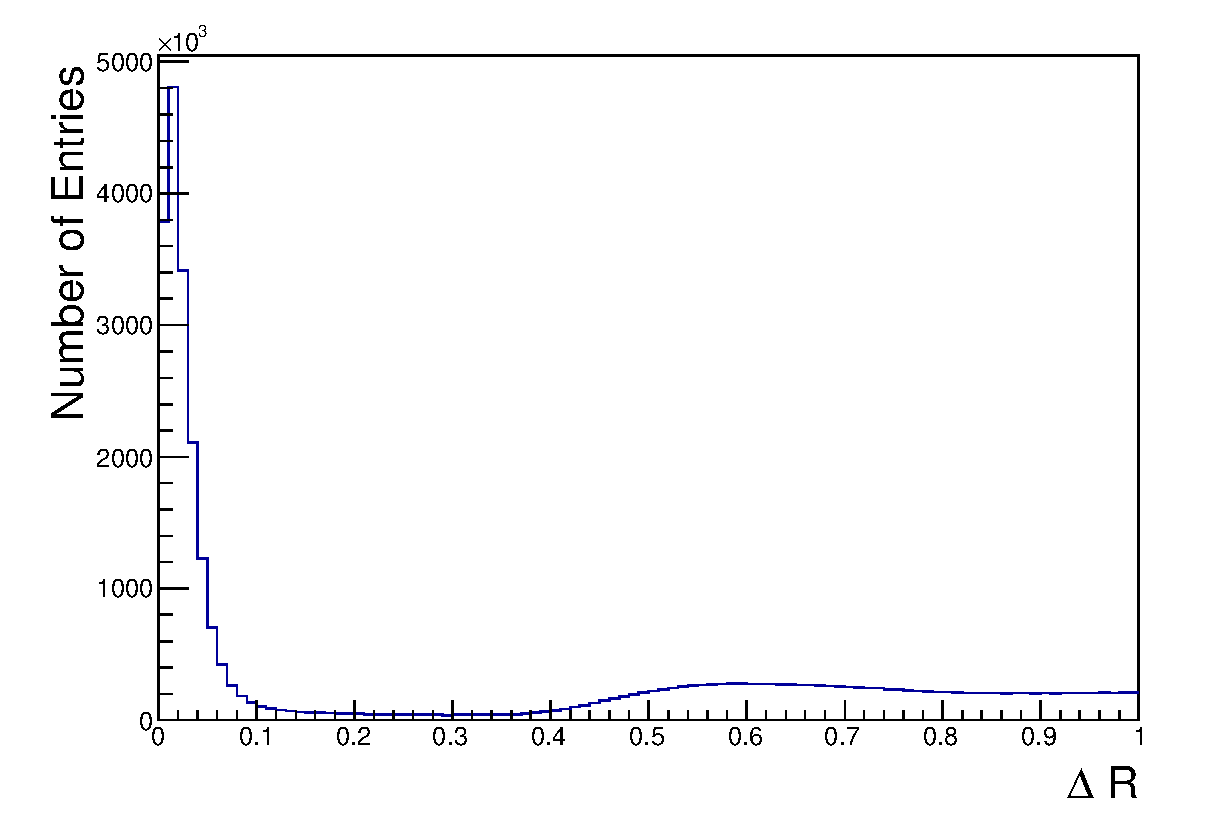
\includegraphics[width=\textwidth]{figures/ServiceWork/Jets/L2_DRUnmatchedJetsZoomedJet.eps}
        \end{subfigure}%
\caption[\dr{} between offline and L2 jets]{
\dr{} distribution between the offline jet and all L2 jets in the event, shown within the range (a) $0 - 6$ and (b) $0 - 1$.
\label{SW_jet_L2_dR}}
\end{figure}

\begin{figure}
\centering
        \begin{subfigure}[b]{0.5\textwidth}
                \centering
                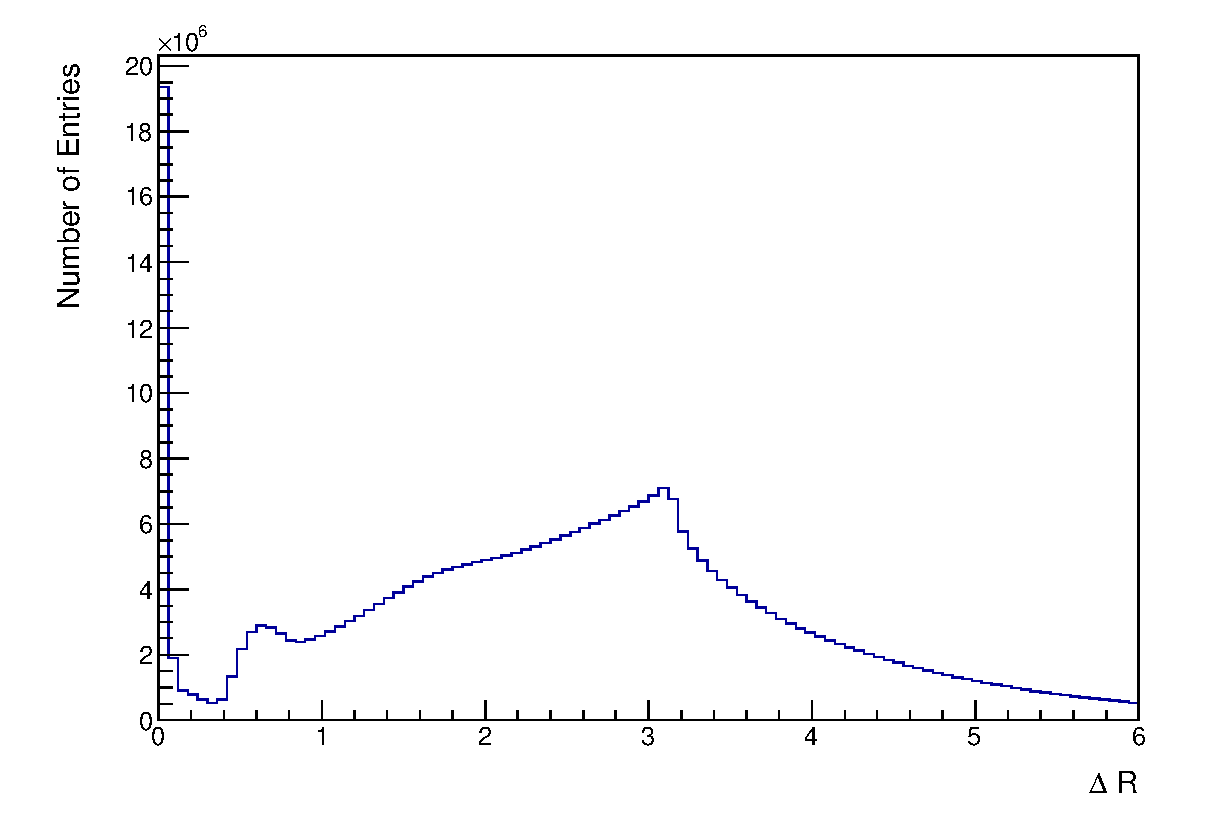
\includegraphics[width=\textwidth]{figures/ServiceWork/Jets/EF_DRUnmatchedJetsJet.eps}
        \end{subfigure}%
        \begin{subfigure}[b]{0.5\textwidth}
                \centering
                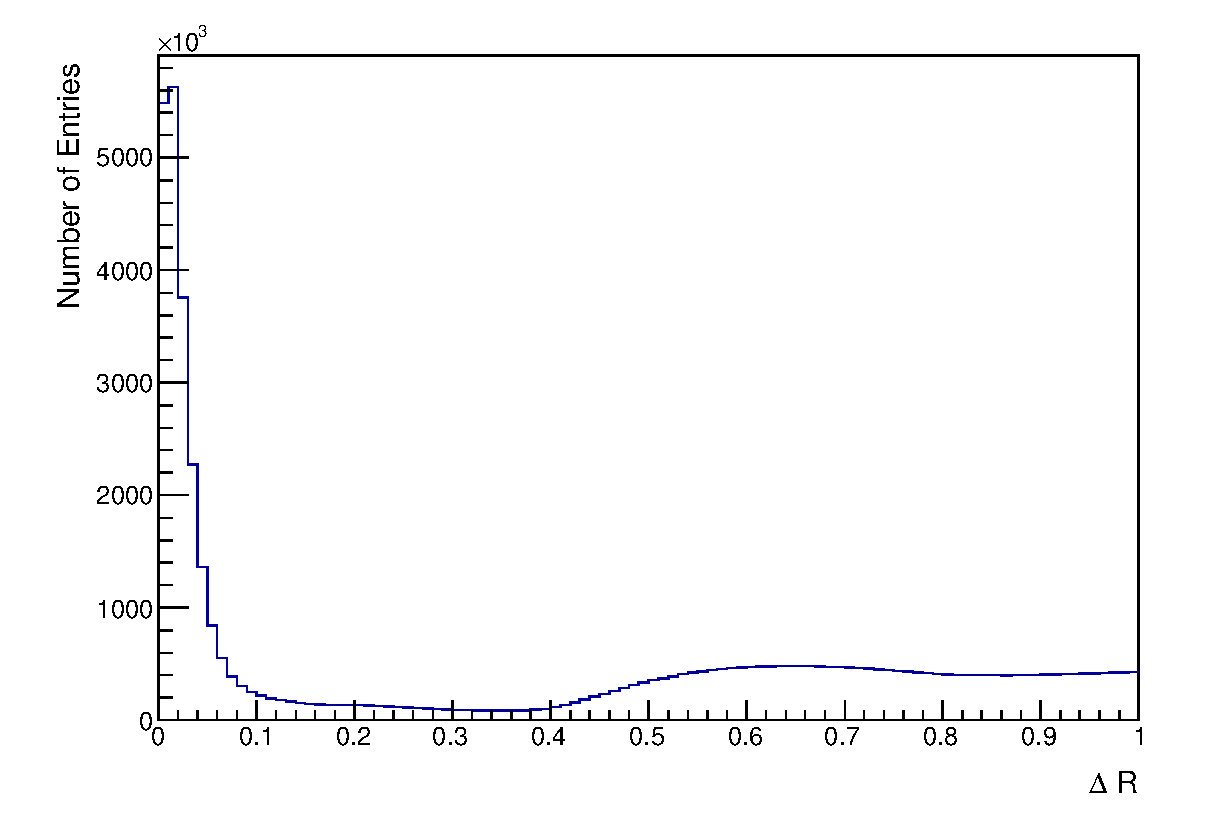
\includegraphics[width=\textwidth]{figures/ServiceWork/Jets/EF_DRUnmatchedJetsZoomedJet.eps}
        \end{subfigure}%
\caption[\dr{} between offline and EF jets]{
\dr{} distribution between the offline jet and all EF jets in the event, shown within the range (a) $0 - 6$ and (b) $0 - 1$.
\label{SW_jet_EF_dR}}
\end{figure}



\subsubsection{Monitored Distributions}

The jet monitoring uses the same distributions as the monitoring of the EM clusters.
The monitoring distributions shown in Figures \ref{SW_jet_L2EF_EtEt} - \ref{SW_jet_L2EF_Reco} are from run 203335, which was taken in 2012.
Figure \ref{SW_jet_L2EF_EtEt} shows the \et{} of the offline jet versus the \et{} of (a) the L2 and (b) the EF jets.
The \et{} comparison is used to check the linearity of the trigger jet \et{} to that of the offline jet.
The L2 trigger \et{} shows linearity to the offline jet \et{}, with the trigger jets \et{} being $\approx 60 \%$ of the offline jet \et{}. 
This is due to the different energy scales of the jets; whilst the offline are fully calibrated, the L2 trigger jets are at EM scale.
The \et{} of the EF jets agree well with the offline jets. 
This improvement is expected due to the calibration done on the EF jets.
Both the EF jets and the L2 jets have good linearity to the offline jet \et{}.

Figure \ref{SW_jet_L2EF_EtFrac_Eta} shows the \et{} fraction (Equation \ref{SW:EtFrac}) as a function of jet $\eta$ for (a) the L2 jets and (b) the EF jets.
The L2 jets have a mean \et{} fraction of $\approx 0.7$, whilst the EF jets have a mean \et{} fraction closer to one.  
This is again explained due to the jet energy scale of the trigger jets.
In both distributions, underlying differences between the trigger jets and offline jets can be seen in different regions of the detector.
The jumps in $f(\et{})$ at $|\eta|\sim1.2$ are due to the transition between the barrel and the tile calorimeters, where large fluctuations in jet \pt{} are anticipated.


Figure \ref{SW_jet_L2EF_Reco} shows the \et{} resolution of (a) the L2 jets and (b) the EF jets. 
As seen in previous figures, the L2 jets are $\approx 70 \%$ of the offline jets, due to the difference in calibration.
The mean of the \et{} resolution of the EF jets is close to zero. 
Problems in the detector should show up in the plot as a change in the mean.



\begin{figure}
\centering
        \begin{subfigure}[b]{0.5\textwidth}
                \centering
                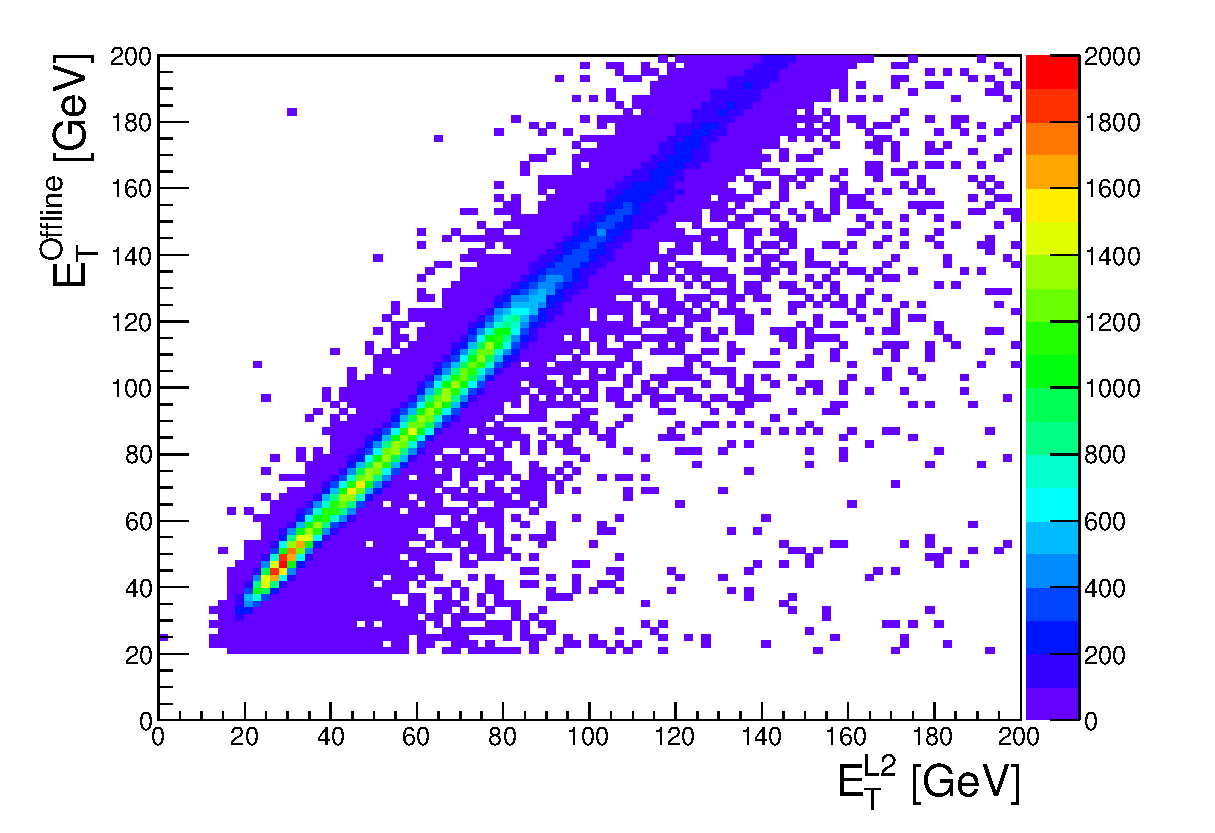
\includegraphics[width=\textwidth]{figures/ServiceWork/Jets/L2_EtEtMatchedJet.eps}
        \end{subfigure}%
        \begin{subfigure}[b]{0.5\textwidth}
                \centering
                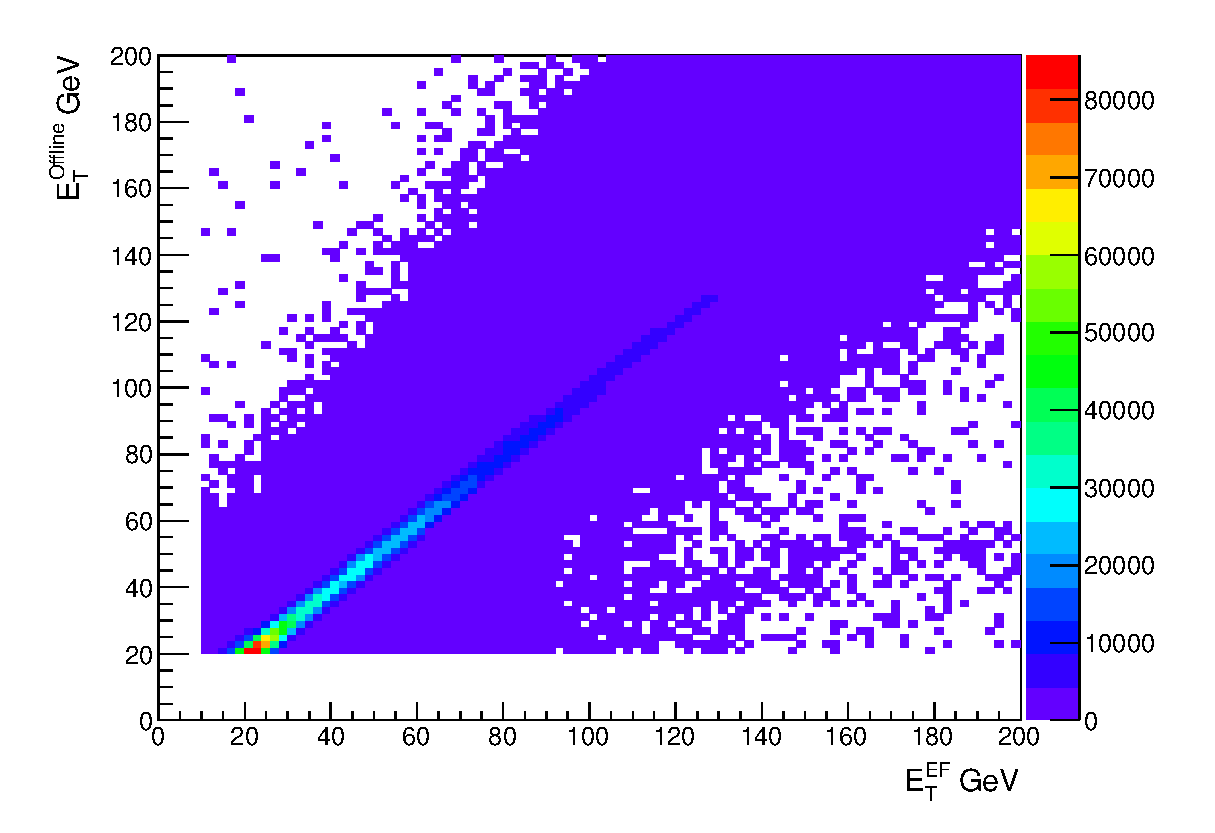
\includegraphics[width=\textwidth]{figures/ServiceWork/Jets/EF_EtEtMatchedJet.eps}
        \end{subfigure}%
\caption[Offline jet \et{} versus L2/EF jet \et{}]{
\et{} of the offline jet versus the \et{} of the matched (a) L2 and (b) EF jet.
\label{SW_jet_L2EF_EtEt}}
\end{figure}


\begin{figure}
\centering
        \begin{subfigure}[b]{0.5\textwidth}
                \centering
                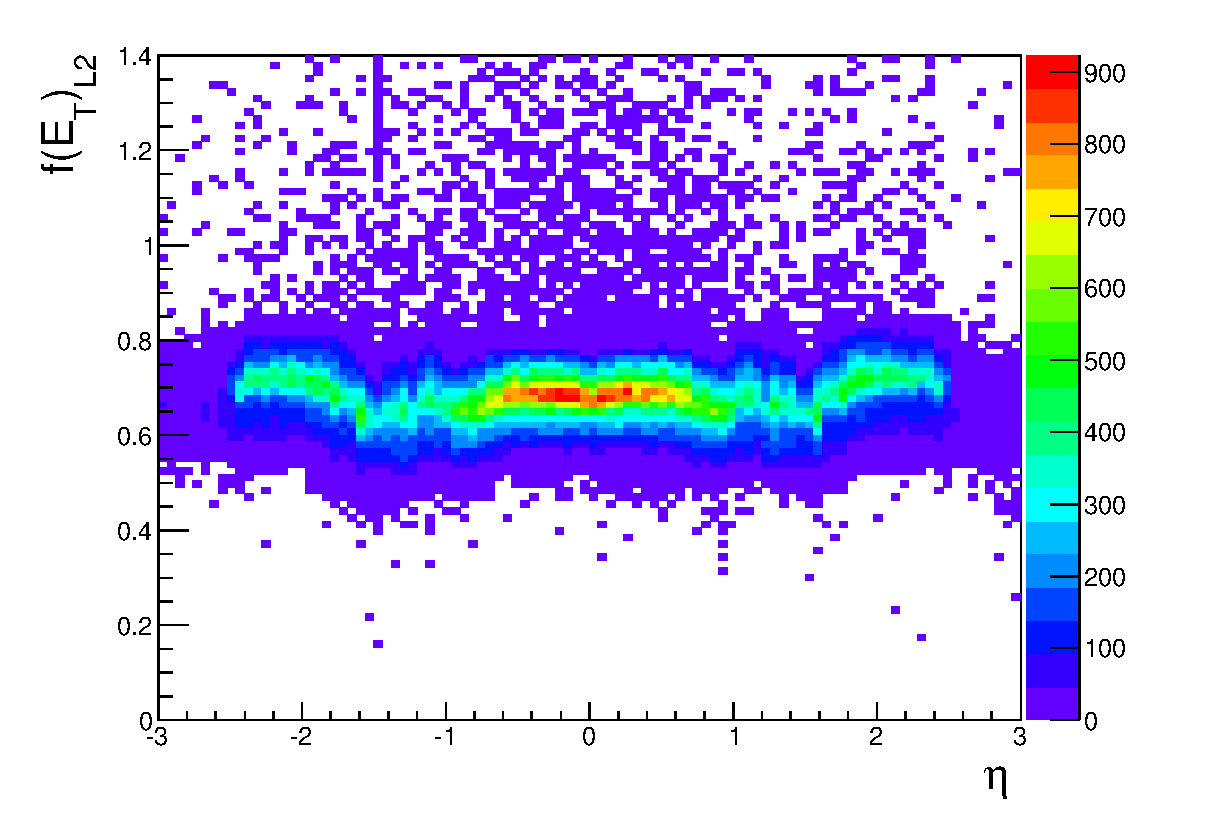
\includegraphics[width=\textwidth]{figures/ServiceWork/Jets/L2_EtFracEtaMatchedJet.eps}
        \end{subfigure}%
        \begin{subfigure}[b]{0.5\textwidth}
                \centering
                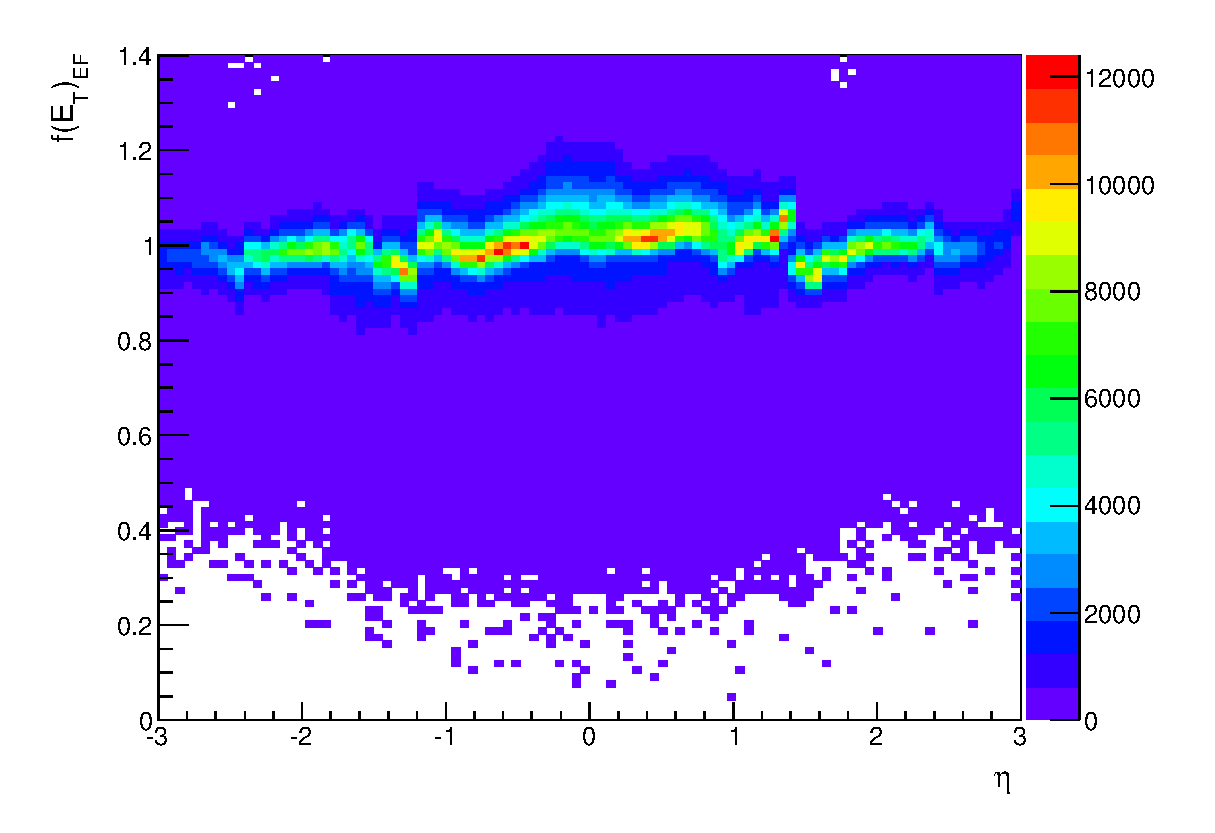
\includegraphics[width=\textwidth]{figures/ServiceWork/Jets/EF_EtFracEtaMatchedJet.eps}
        \end{subfigure}%
\caption[\et{} fraction of L2 and EF jet to offline jet ]{
\et{} fraction of the (a) L2 and (b) EF jets to the offline jet \et{} as a function of $\eta$. 
\label{SW_jet_L2EF_EtFrac_Eta}}

\end{figure}

\begin{figure}
\centering
        \begin{subfigure}[b]{0.5\textwidth}
                \centering
                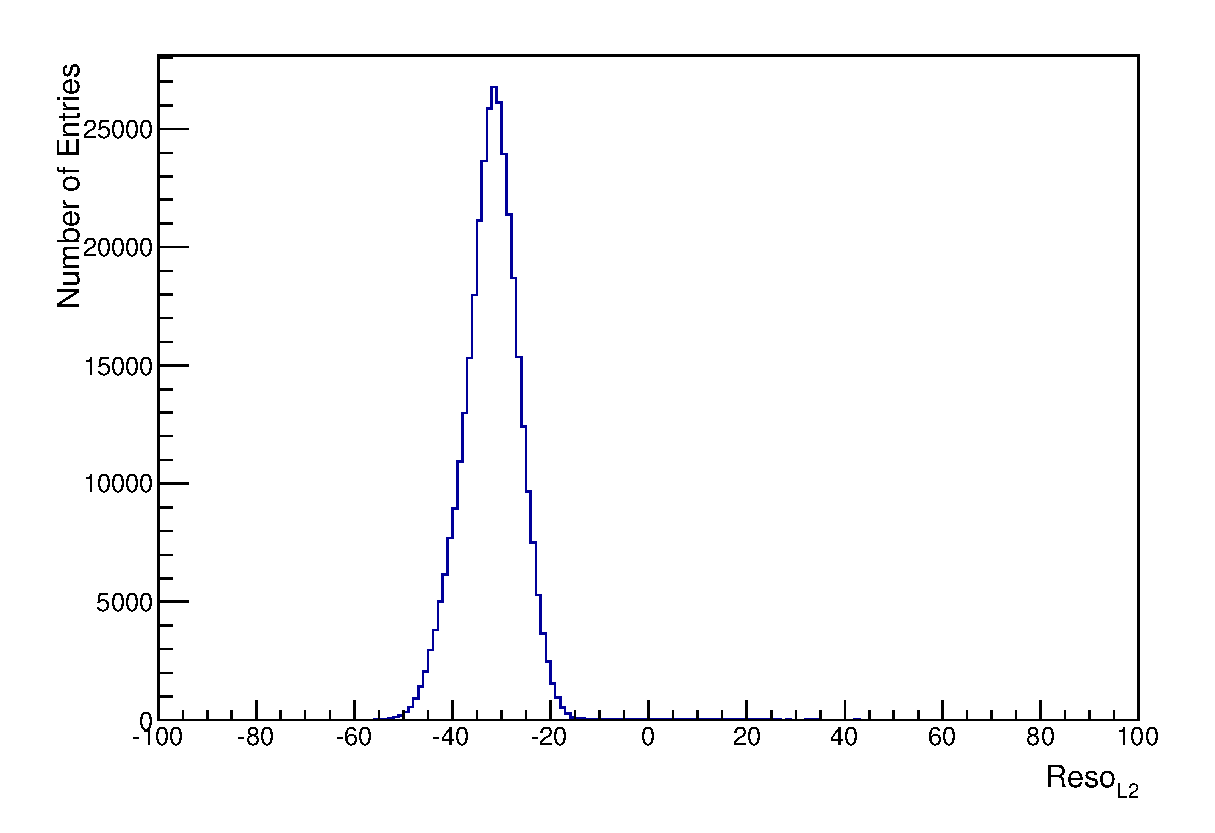
\includegraphics[width=\textwidth]{figures/ServiceWork/Jets/L2_ResoMatchedJetsJet.eps}
        \end{subfigure}%
        \begin{subfigure}[b]{0.5\textwidth}
                \centering
                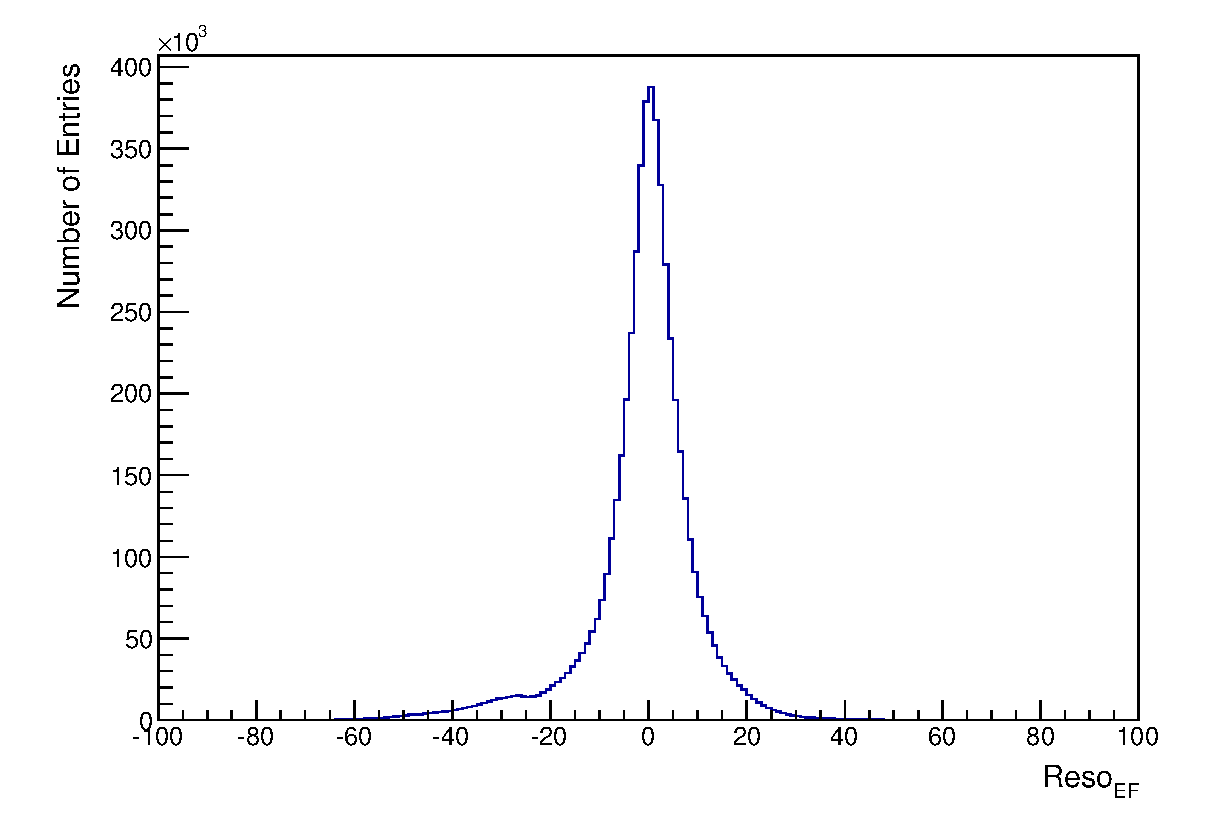
\includegraphics[width=\textwidth]{figures/ServiceWork/Jets/EF_ResoMatchedJetsJet.eps}
        \end{subfigure}%
\caption[\et{} resolution between offline jet \et{} and L2/EF jet \et{}]{
\et{} resolution of (a) the L2 jets and (b) the EF jets. 
\label{SW_jet_L2EF_Reco}}
\end{figure}

